\section{Kd-tree partitioner and dangle and cut edges integration} \label{sec:extension_methods}

\subsubsection{Kd-tree Partition Strategy} \label{sec:kdtreestrategy}
A quadtree data structure follows a space-oriented approach, given that it does not  consider each cell's content at the moment of a possible split.  The kd-tree based partitioning is a data-oriented approach because it sorts and picks the middle point inside a cell to locate the split of the future children.

Building and populating the kd-tree partitioning follows a procedure similar to that of the quadtree, by first building a kd-tree from a sample of the input data.  1\% of the input data is used to build a kd-tree and extract the tree's structure.  The leaves of this structure are the partition's cells.  We feed the input data into the generated kd-tree structure to assign each edge to the leaf cell that has the edge within its boundaries.  After the partitioning is done, the construction of the local DCELs for each layer and the overlay operation is performed in each local cell in the same fashion as described in section \ref{sec:pstrategies}.

In addition to the scalability issue, it is common in some applications that spatial polygons are provided in the form of scattered line segments, e.g., a set of road segments that form city blocks.  Such data can be very large and appear in applications in urban planning, geo-targeted advertising, economic and demographic studies, etc.  Yet, existing polygon overlay techniques cannot handle them directly at scale.  

Section \ref{sec:extension_experiments} will compare two partitioning strategies, the one presented in \ref{sec:pstrategies} based on the quadtree (i.e. space-oriented) and one on the kd-tree (i.e. data-oriented) indexes.  Note that both tree-based data partitioning involves shuffling all edges; this however, happens only once. Our experimental evaluation (see Section \ref{sec:comparison}) shows that the data-oriented approach leads to better performance. 

\subsection{Overlaying Polygons with Dangle and Cut Edges} \label{sec:over_dang}

In this section we extend the overlay method presented in \ref{sec:methods} to support input polygons in scattered line segments form by integrating a scalable and distributed polygon extraction approach supporting the functionality to merge with dangle and cut edges.

 \begin{figure}
    \centering
    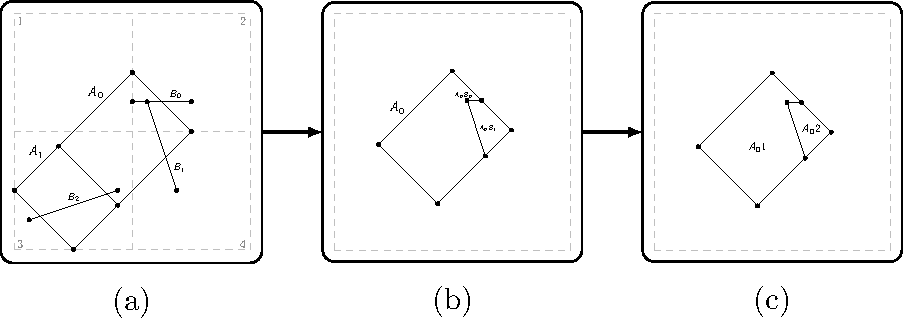
\includegraphics[width=\textwidth]{chapterExtension/dangles_cuts/DAC}
    \caption{(a), (b) and (c).} \label{fig:dangles_cuts}
 \end{figure}
 
We built on in the scalable polygonization procedure presented in \cite{abdelhafeez_ddcel_2023}.  The result of that polygonization procedure produces two outputs: first, a set of closed polygons formed by the input planar line segments, and second, any edges that are not a part of any polygon (i.e., dangle or cut edges).  Overlaying the polygons generated with any polygon layer follows the approaches discussed in sections \ref{sec:methods} and \ref{sec:alternative_methods}.  However, we need to modify the algorithms provided in these previous sections to overlay an input polygon layer $A$ with the dangle and cut edges (layer $B$). In particular, we modify the reduce phase.

Each edge from layer $B$ is labeled a unique label and is fed as an input to the overlay module.  The local overlay is performed by finding intersections between the input polygon layer $A$ and layer $B$ on each data partition.  If a polygon with $id = i$ from polygon layer $A$ intersects with edges with ids $id = a, id = b, id = c$ from layer $B$ at some data partition, we generate a label to match these intersections $A_{i} B_{a} B_{b} B_{c}$.   At the reduce phase, we re-partition the data by the first label, meaning we collect all edges that intersect with the first label.  If two data partitions produced the labels $A_{i} B_{a} B_{b} B_{c}$ and $A_{i} B_{x} B_{y}$, we repartition the data such that $A_{i}$ is on one partition with all edges it is intersecting, i.e., $B_{a}, B_{b}, B_{c}, B_{x}, B_{y}$.

After re-partitioning the data, we have all edges from both layers intersecting each other on the same partition. The next step is to find the polygons generated by these intersections. Since there is no guarantee that only one polygon is generated, we substitute the polygon concatenation proposed in Section \ref{sec:optimizing} by performing \textit{polygonization} on each partition. The polygonization procedure ensures it generates all new possible polygons. The polygonization procedure follows the algorithm presented in \cite{abdelhafeez_ddcel_2023} . It starts with generating the new vertices and half-edges, then marking the current dangles and cut edges, then setting the next pointers, and finally generating the partition polygons. Polygons from all partitions generate the overlay between the polygon layer $A$ and layer $B$.

 \begin{figure}
     \centering
     \begin{tabular}{cc}
         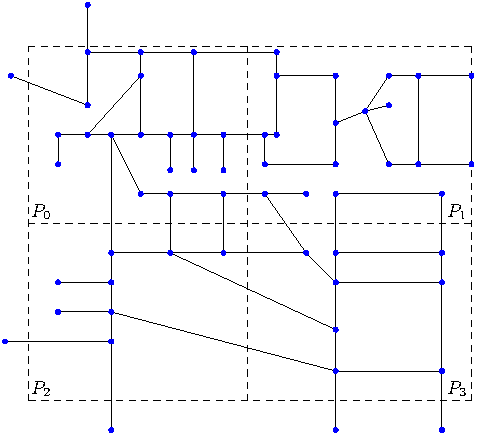
\includegraphics[width=0.49\textwidth]{chapterExtension/model/input/input} &
         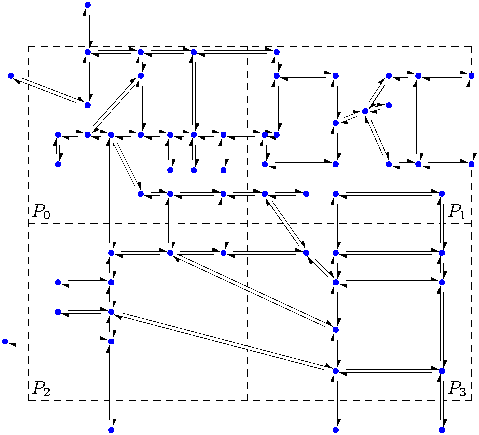
\includegraphics[width=0.49\textwidth]{chapterExtension/model/a/a} \\
         (a) & (b) \\
         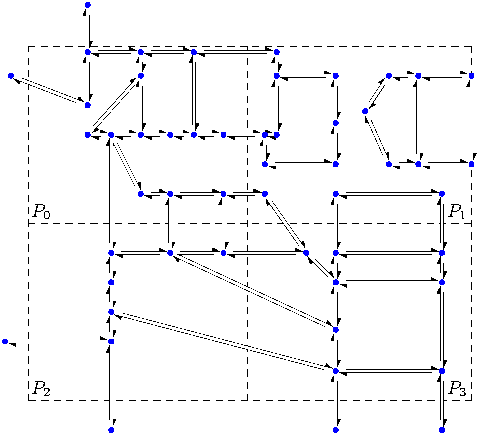
\includegraphics[width=0.49\textwidth]{chapterExtension/model/b/b} &
         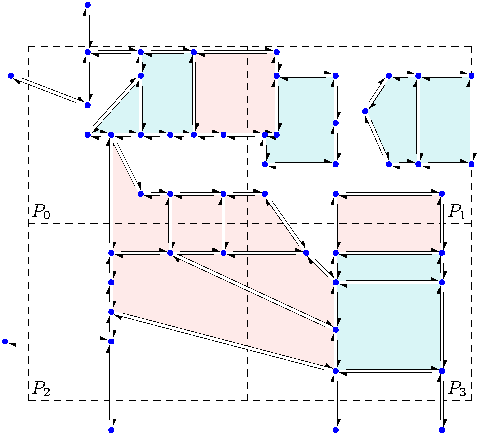
\includegraphics[width=0.49\textwidth]{chapterExtension/model/c/c} \\
         (c) & (d) \\
     \end{tabular}
     \caption{from \cite{abdelhafeez_ddcel_2023}.} \label{fig:polygonization}
 \end{figure}
